\documentclass[simplex.tex]{subfiles}
% NO NEED TO INPUT PREAMBLES HERE
% packages are inherited; you can compile this on its own

\onlyinsubfile{
\title{NeuroData SIMPLEX Report: Subfile}
}

\begin{document}
\onlyinsubfile{
\maketitle
\thispagestyle{empty}

The following report documents the progress made by the labs of Randal~Burns and Joshua~T.~Vogelstein at Johns Hopkins University towards goals set by the DARPA SIMPLEX grant.

%%%% Table of Contents
\tableofcontents

%%%% Publications
\bibliographystyle{IEEEtran}
\begin{spacing}{0.5}
\section*{Publications, Presentations, and Talks}
\vspace{-20pt}
\nocite{*}
{\footnotesize	\bibliography{simplex}}
\end{spacing}
%%%% End Publications
}


\subsection{ndmg}

We have continued the development of a reliable DWI and fMRI processing pipeline
package, with current emphasis on performing intermediate derivative quality
control. The quality of claims made from derived data products is heavily
dependent upon the quality of input data to each processing step. To that end,
it is necessary to perform quality control at each processing step of the
pipelines including: registration, tensor estimation, and fiber estimation. We
generate quality control images for a qualitative analysis enabling the user to
evaluate the quality of derivatives produced (see, Figure \ref{fig:ndmg}). Quality
control is essential to ensure accuracy of and to substantiate claims derived
from ndmg results. In particular, investigating quality control figures has led
to impactful improvements in the diffusion pipeline, which now is nearly
perfectly discriminable for a variety of datasets tested. Moreover, we are
developing a web service for fMRI uploading to streamline the process of
analysis. Our web service will facilitate the dissemination of results and
ensure that researchers have easy access to to a substantial array of
pre-processed data as well as metrics computed upon them.


\begin{figure}[h!]
\begin{cframed}
\centering
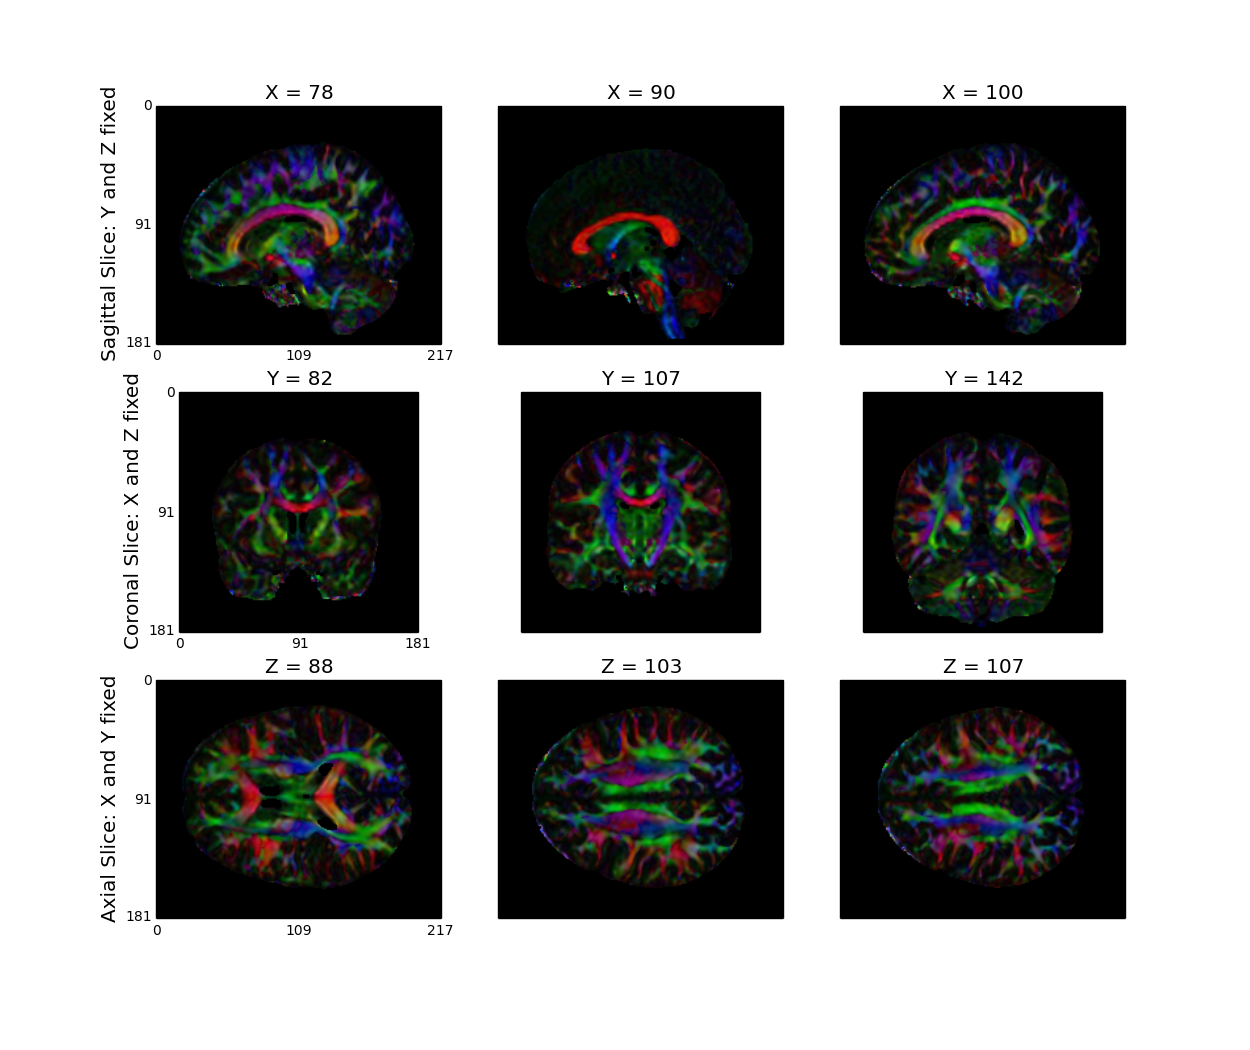
\includegraphics[width=0.85\textwidth]{./figs/ndmg.png}
\caption{
NDMG various output views.  
}
\label{fig:ndmg}
\end{cframed}
\end{figure}
\end{document}
